\documentclass[UTF8]{article}
\usepackage{bm}
\usepackage{amsmath}
\usepackage{cases}
\usepackage{cite}
\usepackage{graphicx}
\usepackage[margin=1in]{geometry}
\geometry{a4paper}
\usepackage{fancyhdr}
\usepackage{array}
\pagestyle{fancy}
\usepackage{wrapfig}
\fancyhf{}
\usepackage{float}  %设置图片浮动位置的宏包
\usepackage{subfigure}
\usepackage{caption}
\usepackage{booktabs}
\usepackage{listings}
\usepackage{xcolor}
\usepackage{multirow}
\lstset{numbers=left, %设置行号位置
	numberstyle=\tiny, %设置行号大小
	keywordstyle=\color{blue}, %设置关键字颜色
	commentstyle=\color[cmyk]{1,0,1,0}, %设置注释颜色
	frame=single, %设置边框格式
	escapeinside=``, %逃逸字符(1左面的键),用于显示中文
	breaklines, %自动折行
	extendedchars=false, %解决代码跨页时,章节标题,页眉等汉字不显示的问题
	xleftmargin=2em,xrightmargin=2em, aboveskip=1em, %设置边距
	tabsize=4, %设置tab空格数
	showspaces=false %不显示空格
}

\title{Dual grating weak vibration measurement}
\author{by 22 Artificial Intelligence ChenxuZhang}
\date{2023.6.05}
\pagenumbering{arabic}

\begin{document}
	
	\fancyhead[L]{ChenxuZhang}
	\fancyhead[R]{ID 202264691028}
	\fancyfoot[C]{\thepage}
	
	\maketitle
	\tableofcontents
	\newpage
	
	\section{Abstract}
 The physical properties of Doppler shift are also used in a wide range of applications, such as ultrasound diagnostic instruments in medicine, measuring the speed and direction of seawater currents at various depths, satellite navigation systems, tuning of musical instruments, etc. The Doppler frequency shift physical properties are also used in a wide range of applications, such as ultrasonic diagnostic instruments in medicine, measuring the speed and direction of seawater currents at various depths, satellite navigation and positioning systems, and tuning musical instruments. Double grating weak vibration measurement instrument is used in mechanical experimental projects as tuning fork vibration analysis, weak amplitude (displacement), measurement and optical beat research.

In the process of electromagnetic wave propagation, due to the relative motion between the light source and the receiver so that the receiver receives a light wave frequency different from that of the light emitted by the light source is called the Doppler effect, the resulting change in frequency is called Doppler frequency shift. If a moving grating moves relative to a stationary grating, the laser beam passing through such a double grating can produce the Doppler effect of light. Doppler effect, the frequency shift and non-frequency shift of the two beams directly parallel superposition can be obtained light beat, and then through the photoelectric square law. Detector detection, take out the differential frequency signal, you can accurately measure the displacement of the weak vibration.
 
	
\section{Purpose of the experiment}
   $\bm{A}$.To understand the principle of using the Doppler shift of light to form an optical beat and use it to measure the optical beat frequency.\\
   $\bm{B}$.Learn to use a method for accurately measuring the displacement of weak vibrations.\\
   $\bm{C}$.Apply the dual grating weak vibration measurement instrument to measure the microamplitude of tuning fork vibration.

	\section{Experimental apparatus}
	Laser source, signal generator, frequency meter (the above instruments have been integrated in the measuring instrument case)
	\begin{figure}[H]
	    	\centering
	    	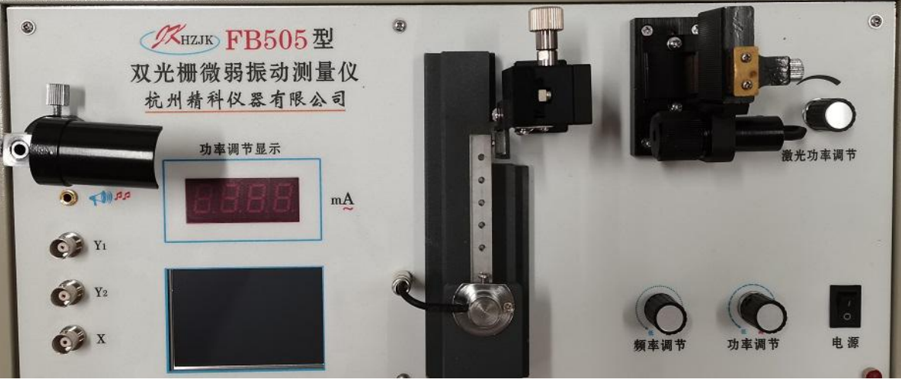
\includegraphics[clip,scale=1,trim={0 0 0 0}]{fig/fig1.png}
	        \caption{Dual grating weak vibration measurement panel structure}
	        \label{figure.1}
    \end{figure}
	
	
	\begin{itemize}
	\item \textbf{Laser Source}: A device that emits a coherent and focused beam of light through the process of stimulated emission. It is commonly used in various applications such as research, telecommunications, and industrial processes.
	
	\item \textbf{Signal Generator}: An electronic device used to generate electrical waveforms of different frequencies, amplitudes, and shapes. It is commonly used in testing, troubleshooting, and design of electronic circuits and systems.
	
	\item \textbf{Frequency Counter}: A device used to measure the frequency of a periodic waveform. It counts the number of cycles or pulses within a specific time period and displays the result in hertz (Hz) or other frequency units. It is commonly used in electronic testing, telecommunications, and scientific research.
	\end{itemize}
    
        
	\section{Experimental principles}   
    \subsection{Doppler shift of a moving optical phase grating}
    By phase objects we mean transparent bodies that have only a spatial phase structure and the same transparency, such as biological cut sheets, oil films, thermoplastics, etc., which only change the phase of the incident light without affecting its amplitude. When a laser plane wave is perpendicularly When a laser plane wave is incident on a phase grating, the incident plane wave is delayed by the phase delay due to the different optical densities and light sparse media parts on the phase grating. The incident plane wave is transformed into a folded wavefront at the exit, due to the phase delay effect of the different optical densities and optical sparse media parts on the phase grating.
	\begin{figure}[H]
	    	\centering
	    	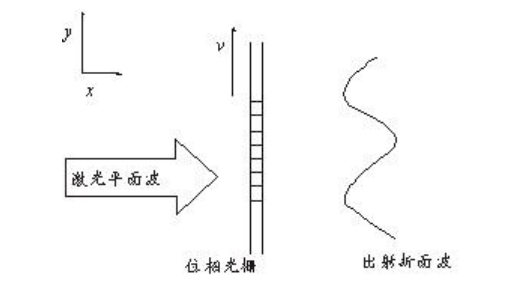
\includegraphics[clip,scale=1,trim={0 0 0 0}]{fig/fig2.png}
	        \caption{Outgoing Folded Wave Front}
	        \label{figure.2}
    \end{figure}  
    
   The intensity of light passing through a grating appears to change periodically due to the diffraction of the single slit on the grating itself and the interference between the slits. In the far field, we can use the familiar grating diffraction equation to express the position of the main maximum as follows:
   \begin{eqnarray}
   d\sin \theta =\pm k\lambda \qquad k=0,1,2,3,\cdots 
   \end{eqnarray}
   
  where: the integer $k$ is the principal great magnitude, $d$ is the grating constant, $\theta$ is the diffraction angle, and $\lambda$ is the wavelength of the light wave.
  
  If the grating moves with velocity $v$ in the y-direction, the wavefront plane of light exiting from the grating also moves with velocity $v$ in the y-direction. Therefore, at different moments, for the same level of diffraction, it also has a displacement of $vt$ in the $y$ direction when it exits from the grating, see Fig:
	\begin{figure}[H]
	    	\centering
	    	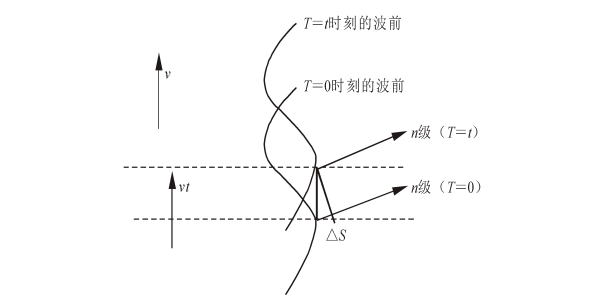
\includegraphics[clip,scale=1,trim={0 0 0 0}]{fig/fig3.png}
	        \caption{Displacement of the diffracted ray in the y-direction}
	        \label{figure.3}
    \end{figure} 
   
   This displacement corresponds to the change of the outgoing optical wave potential phase as$\Delta \phi (t)$:
   \begin{eqnarray}
   \Delta \phi(t)=\frac{2 \pi}{\lambda} \Delta s=\frac{2 \pi}{\lambda} v t \sin \theta
   \end{eqnarray}
   
   Substituting the equation into the graph gives:
   \begin{eqnarray}
   \Delta \phi(t)=\frac{2 \pi}{\lambda} v t \frac{k \lambda}{d}=k 2 \pi \frac{v}{d} t=k \omega_{d} t
   \end{eqnarray}
   
   If a laser is emitted from a stationary grating, the light wave electric vector equation is:
   \begin{eqnarray}
   E=E_{0} \cos \omega_{0} t
   \end{eqnarray}
   
   And when the laser is emitted from the corresponding moving grating, the light wave electric vector equation is:
   \begin{eqnarray}
   E=E_{0} \cos \left[\omega_{0} t+\Delta \phi(t)\right]=E_{0} \cos \left[\left(\omega_{0}+k \omega_{d}\right) t\right]
   \end{eqnarray}
   
   It is obvious that the moving k-level diffracted light wave of the phase grating has a Doppler shift with respect to the stationary phase grating with a frequency of :
   \begin{eqnarray}
   \omega_{D}=\omega_{0}+k \omega_{d}
   \end{eqnarray}
   
   \subsection{Light shot acquisition and detection}
   \subsubsection{Detection of light shot}
   The optical frequency is very high, in order to detect the Doppler shift in the optical frequency, we must use the method of "beat", that is, the frequency-shifted and not frequency-shifted beams are iterated in parallel to each other to form a light beat. Because the beat frequency is low, easy to measure, through the beat frequency can be detected Doppler shift.
   In this experiment, two identical gratings are used in parallel, one B is stationary and the other A is moving relative to each other. The diffracted light formed by the laser passing through the double grating is the parallel iteration of two or more beams. The Doppler shift of the kth level diffracted light wave is shown in the figure.
   \begin{figure}[H]
      \begin{minipage}[t]{0.5\linewidth}
         \centering
         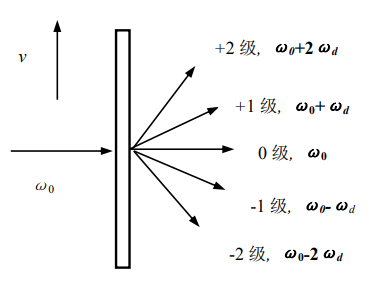
\includegraphics[clip,scale=1,trim={0 0 0 0}]{fig/fig4.png}
         \label{figure.4}
         \caption{Mobile grating for more}
      \end{minipage}
      \begin{minipage}[t]{0.5\linewidth}
         \centering
         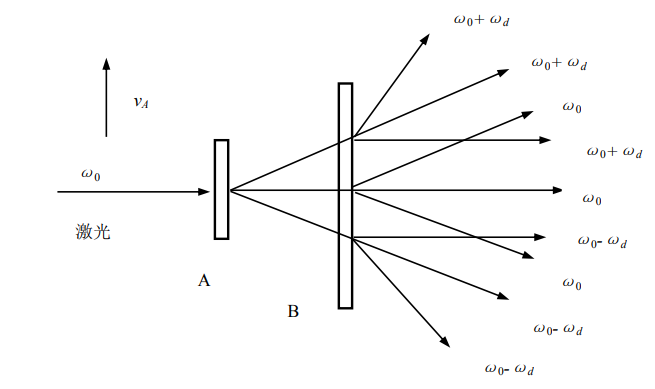
\includegraphics[clip,scale=0.7,trim={0 0 10 0}]{fig/fig5.png}
         \label{figure.5}
         \caption{Doppler shift of k-level diffracted light waves}
      \end{minipage}
      	  
   \end{figure} 
   The grating $A$ moves at the speed $D$ and plays the role of frequency shift, while the grating $B$ is stationary and only plays the role of diffraction, so the diffracted light emitted through the double grating contains more than two different frequency components and parallel beams. Due to the double grating close, the laser has a certain width, and the grating constant $d$ relative to the wavelength of the light wave into a large, so the same line of light spot beam can be parallel iteration, so directly and simply formed a light beat.
   
   When the laser through the double grating formed by the shot superimposed into light beat signal, light beat signal into the photodetector, its output current can be obtained from the following relationship:
   
   Let the electric vector of beam 1 be:
   \begin{eqnarray}
   E_{1}=E_{10} \cos \left(\omega_{0} t+\varphi_{1}\right)
   \end{eqnarray}
   
   The electric vector of beam 2 is:
   \begin{eqnarray}
   \left.E_{2}=E_{20} \cos \left[\left(\omega_{0}+\omega_{d}\right) t+\varphi_{2}\right)\right]
   \end{eqnarray}
   
   Taking k = 1, the photocurrent I:
   \begin{eqnarray}
   \begin{matrix}
   I=\xi\left(E_{1}+E_{2}\right)^{2} = \\
  \xi\left\{E_{10}^{2} \cos ^{2}\left(\omega_{0} t+\varphi_{1}\right)+E_{20}^{2} \cos ^{2}\left[\left(\omega_{0}+\omega_{d}\right) t+\varphi_{2}\right]+\right. \\
   E_{10} E_{20} \cos \left[\left(\omega_{0}+\omega_{d}-\omega_{0}\right) t+\left(\varphi_{2}-\varphi_{1}\right)\right]+ \\
   \left.E_{10} E_{20} \cos \left[\left(\omega_{0}+\omega_{d}+\omega_{0}\right) t+\left(\varphi_{2}+\varphi_{1}\right)\right]\right\}
   \end{matrix}
      \end{eqnarray}
      
   Where $\delta $ is the photoelectric conversion constant.
      
   Because the light wave frequency $\omega _0$ is very high, in the first, second, four, photoelectric detector can not respond, the third term that is the beat frequency signal, because the frequency is low, photoelectric detector can make the corresponding response, the photocurrent is:
   \begin{eqnarray}
   i_{S}=\xi\left\{E_{10} E_{20} \cos \left[\omega_{d} t+\left(\varphi_{2}-\varphi_{1}\right)\right]\right\}
   \end{eqnarray}   
   
   Therefore, the photodetector can detect the frequency of the light beat signal is the beat frequency $F$ beat:
   \begin{eqnarray}
   F_{\text {beat }}=\frac{\omega_{d}}{2 \pi}=\frac{v_{A}}{d}=v_{A} n_{\theta}
   \end{eqnarray}
   
   Where $n_{\theta}=1/d$ is the grating density. In this experiment, $n_{\theta}=100$ bars/mm.
   
   \subsubsection{Detection of weak vibration displacement}
   From the above formula can be seen, $F_ {\text{beat}}$ and light frequency $\omega _{\theta } $ independent, and when the grating density $n_{\theta}$ is a constant, only proportional to the grating moving speed $v_A$, if the grating is glued to the tuning fork, then $v_A$ is periodically changing, so the light beat signal frequency $F_ {\text{beat}}$ is also changing with time, the displacement amplitude of the faint vibration is:
   \begin{eqnarray}
   A=\frac{1}{2} \int_{0}^{T / 2} v(t) d t=\frac{1}{2} \int_{0}^{T / 2} \frac{F_{\text {beat }}(t)}{n_{\theta}} d t=\frac{1}{2 n_{\theta}} \int_{0}^{T / 2} F_{\text {beat }}(t) d t
   \end{eqnarray}
   
   Where $T$ is the period of tuning fork vibration and $ \int_{0}^{T / 2} F_{\text {beat }}(t) d t$ represents the number of waveforms of beat frequency waves in $T/2$ time. Therefore, the displacement amplitude of the weaker vibration can be obtained by measuring the waveform number of beat frequency waveform.
   	\begin{figure}[H]
   	    	\centering
   	    	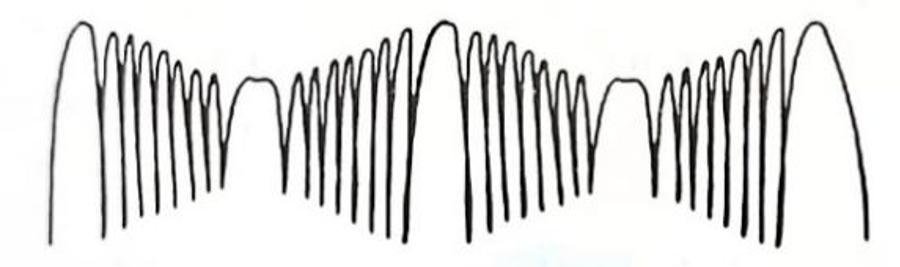
\includegraphics[clip,scale=1,trim={0 0 0 0}]{fig/fig6.png}
   	        \caption{Oscilloscope showing beat frequency waveform}
   	        \label{figure.6}
       \end{figure} 
       
   The waveform number consists of three parts: the number of complete waveforms, the first number of waves, and the last number of waves. It is calculated from the display on the oscilloscope as:
   \begin{eqnarray}
   \text { Waveform number }=\text { Integer waveform number }+\frac{a}{l}+\frac{b}{l}
   \end{eqnarray}
   
   where $a$ and $b$ are the lengths of the first and last parts of the wave group, respectively, and $l$ is the average length of a complete waveform.
       
       
	\section{Contents and Steps}
	Next we will complete the experiment by following the following steps:
	\begin{itemize}
	\item Connect the external triggers of Y1, Y2, and X of the oscilloscope to the output sockets of Y1, Y2, and X of the double grating weak vibration measuring instrument, and turn on their power supply.
	\item Geometric optical path adjustment:
	\begin{itemize}
	\item Adjust the laser fixer to make the red laser pass through the static grating and moving grating.
	\item Let a level of diffracted light just fall into the small hole in front of the photocell.
	\end{itemize}
	\item Tuning fork resonant adjustment:
	\begin{itemize}
	\item Adjust the "power" knob to make the output power about 45mA.
	\item Adjust the "frequency" coarse adjustment knob to make the frequency about 508Hz.
	\item Adjust the "frequency" fine-tuning knob to make the tuning fork resonate.
	\item Use an available ear test to find the adjustment direction.
	\item If the tuning fork resonance is too strong, turn the "power" knob in the direction of the smaller hour to make the maximum wave number of the light beat in T/2 seen on the oscilloscope.
	\item Record the vibration frequency of the tuning fork at this time, the number of complete waves on the screen, the beginning and mantissa values of less than a complete waveform, and the amplitude of the corresponding complete waveform.
	\end{itemize}
	\item Measurement of the harmonic curve of the tuning fork driven by external force:
	\begin{itemize}
	\item Fix the position of the "power" knob.
	\item Carefully adjust the "frequency" knob near the tuning fork resonance point.
	\item Measure the vibration frequency of the tuning fork and the corresponding signal amplitude.
	\item The frequency interval can be 0.1Hz, select 8 points, measure the number of corresponding waves respectively, and record the data in the table.
	\item The amplitude $A = \frac{N}{2n_\theta}$ is calculated by the amplitude formula, where $N$ is the wave number in the upper half cycle of the oscilloscope.
	\end{itemize}
	\item Cause the tuning fork to vibrate at a frequency near resonance:
	\begin{itemize}
	\item Start the output power from 10mA.
	\item Measure the tuning fork amplitude under the action of the output power of each signal.
	\item Measure the relationship between tuning fork power and tuning fork amplitude.
	\item Record the data in a table.
	\end{itemize}
	\item Note: The laser power is generally adjusted to the middle and does not need to be adjusted frequently. When counting the wave number of the beat frequency wave on the fluorescent screen of the oscilloscope, it is better to wait until the waveform is stable.
	\end{itemize}
    
	
	\section{Data processing}
    First we obtained the following basic data by commissioning and measuring the experimental equipment, including the resonant frequency of the tuning fork, the displacement amplitude at the resonance point:
    \begin{itemize}
    \item Tuning fork resonant frequency: $f = 508.406  \text{Hz}$.
    \item The tuning fork at the resonant point for weak vibration displacement amplitude: $A = 0.10  \text{mm}$.
    \end{itemize}
    
    Next we hold the power constant, adjust the frequency and record the change in waveform number and amplitude in this case, as shown in the table below:
    \begin{table}[htbp]
      \centering
      \caption{Variation of amplitude with frequency}
        \begin{tabular}{rrr}
         \toprule[2pt]
        \multicolumn{1}{l}{\textcolor[rgb]{0.165, 0.169, 0.180}{frequency}} & \multicolumn{1}{l}{Number of waveforms} & \multicolumn{1}{l}{Calculate amplitude} \\
        \midrule
        508.106 & 4     & 0.02032424 \\
        508.206 & 5     & 0.0254103 \\
        508.306 & 12    & 0.06099672 \\
        508.406 & 19    & 0.09659714 \\
        508.506 & 10    & 0.0508506 \\
        508.606 & 6     & 0.03051636 \\
        508.706 & 4     & 0.02034824 \\
        \bottomrule[2pt]
        \end{tabular}%
      \label{tab:addlabel}%
    \end{table}%
    
    Based on the above data we can draw the following graphs:
    	\begin{figure}[H]
       	    	\centering
       	    	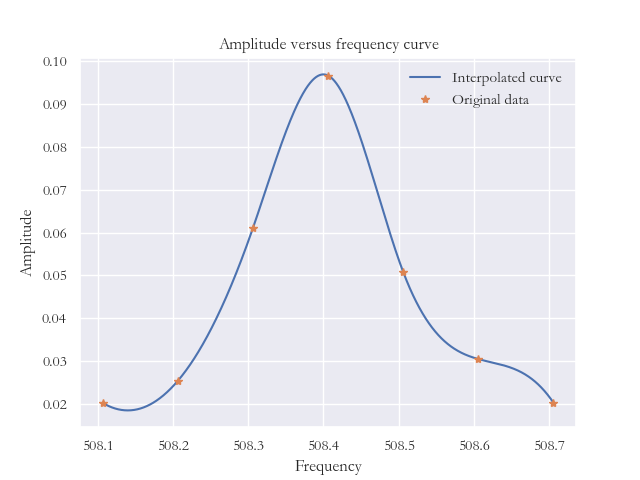
\includegraphics[clip,scale=1,trim={0 0 0 0}]{fig/fig7.png}
       	        \caption{Amplitude versus frequency curve}
       	        \label{figure.7}
           \end{figure}
           
    We then tried to keep the frequency of the vibration constant and vary the output power, recording the change in waveform number and amplitude with this adjustment:
    \begin{table}[htbp]
      \centering
      \caption{Add caption}
        \begin{tabular}{rrrr}
        \toprule[2pt]
        \multicolumn{1}{l}{Power} & \multicolumn{1}{l}{Number of waveforms} & \multicolumn{1}{l}{Calculate amplitude} & \multicolumn{1}{l}{Signal amplitude} \\
        \midrule
        10    & 5     & 0.0254203 & 84 \\
        20    & 9     & 0.04575654 & 40 \\
        30    & 11    & 0.05592466 & 62 \\
        40    & 19    & 0.09659714 & 65 \\
        50    & 22    & 0.11184932 & 108 \\
        60    & 27    & 0.13726962 & 42 \\
        70    & 29    & 0.14743774 & 72 \\
        80    & 30    & 0.1525218 & 73 \\
        90    & 30    & 0.1525218 & 72 \\
        100   & 31    & 0.15760586 & 70 \\
        \bottomrule[2pt]
        \end{tabular}%
      \label{tab:addlabel}%
    \end{table}%
    
    Based on the above data we can draw the following graphs:
    \begin{figure}[H]
           	    	\centering
           	    	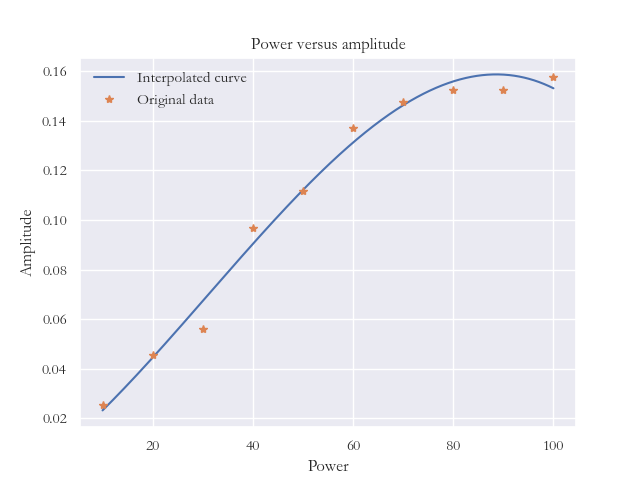
\includegraphics[clip,scale=1,trim={0 0 0 0}]{fig/fig8.png}
           	        \caption{Power versus amplitude}
           	        \label{figure.8}
    \end{figure}

\section{Conclusion and analysis}
\subsection{Conclusion}
The experimental results show that the dual grating method of measuring weak vibration has high accuracy, high sensitivity and high reliability, and can be used for various weak vibration measurements.

\subsection{Error analysis}
\begin{itemize}
  \item \textbf{Environmental vibration:} The presence of vibration in the laboratory environment may interfere with the experiment. These vibrations can come from equipment operation, personnel activity, air conditioning systems, or vibrations in the surrounding environment. Such vibrations can cause small changes in the position of the grating, which can affect the measurement results.
  
  \item\textbf{ Light source instability:} Instability of the light source may lead to fluctuations in light intensity, which can affect the measurement results. For example, if the brightness or frequency of the light source changes, it will have an impact on the interference pattern, resulting in measurement errors.
  
  \item \textbf{Optical system errors:} Components in the optical system, such as lenses, mirrors, optical fibers, etc., may have manufacturing or calibration errors. These errors may lead to distortion, shift, or divergence of the beam, which in turn affects the accuracy of the measurement results.
\end{itemize}

\end{document}  